% Options for packages loaded elsewhere
\PassOptionsToPackage{unicode}{hyperref}
\PassOptionsToPackage{hyphens}{url}
%
\documentclass[
  ignorenonframetext,
]{beamer}
\usepackage{pgfpages}
\setbeamertemplate{caption}[numbered]
\setbeamertemplate{caption label separator}{: }
\setbeamercolor{caption name}{fg=normal text.fg}
\beamertemplatenavigationsymbolsempty
% Prevent slide breaks in the middle of a paragraph
\widowpenalties 1 10000
\raggedbottom
\setbeamertemplate{part page}{
  \centering
  \begin{beamercolorbox}[sep=16pt,center]{part title}
    \usebeamerfont{part title}\insertpart\par
  \end{beamercolorbox}
}
\setbeamertemplate{section page}{
  \centering
  \begin{beamercolorbox}[sep=12pt,center]{part title}
    \usebeamerfont{section title}\insertsection\par
  \end{beamercolorbox}
}
\setbeamertemplate{subsection page}{
  \centering
  \begin{beamercolorbox}[sep=8pt,center]{part title}
    \usebeamerfont{subsection title}\insertsubsection\par
  \end{beamercolorbox}
}
\AtBeginPart{
  \frame{\partpage}
}
\AtBeginSection{
  \ifbibliography
  \else
    \frame{\sectionpage}
  \fi
}
\AtBeginSubsection{
  \frame{\subsectionpage}
}
\usepackage{amsmath,amssymb}
\usepackage{lmodern}
\usepackage{ifxetex,ifluatex}
\ifnum 0\ifxetex 1\fi\ifluatex 1\fi=0 % if pdftex
  \usepackage[T1]{fontenc}
  \usepackage[utf8]{inputenc}
  \usepackage{textcomp} % provide euro and other symbols
\else % if luatex or xetex
  \usepackage{unicode-math}
  \defaultfontfeatures{Scale=MatchLowercase}
  \defaultfontfeatures[\rmfamily]{Ligatures=TeX,Scale=1}
\fi
\usecolortheme{beaver}
% Use upquote if available, for straight quotes in verbatim environments
\IfFileExists{upquote.sty}{\usepackage{upquote}}{}
\IfFileExists{microtype.sty}{% use microtype if available
  \usepackage[]{microtype}
  \UseMicrotypeSet[protrusion]{basicmath} % disable protrusion for tt fonts
}{}
\makeatletter
\@ifundefined{KOMAClassName}{% if non-KOMA class
  \IfFileExists{parskip.sty}{%
    \usepackage{parskip}
  }{% else
    \setlength{\parindent}{0pt}
    \setlength{\parskip}{6pt plus 2pt minus 1pt}}
}{% if KOMA class
  \KOMAoptions{parskip=half}}
\makeatother
\usepackage{xcolor}
\IfFileExists{xurl.sty}{\usepackage{xurl}}{} % add URL line breaks if available
\IfFileExists{bookmark.sty}{\usepackage{bookmark}}{\usepackage{hyperref}}
\hypersetup{
  hidelinks,
  pdfcreator={LaTeX via pandoc}}
\urlstyle{same} % disable monospaced font for URLs
\newif\ifbibliography
\setlength{\emergencystretch}{3em} % prevent overfull lines
\providecommand{\tightlist}{%
  \setlength{\itemsep}{0pt}\setlength{\parskip}{0pt}}
\setcounter{secnumdepth}{-\maxdimen} % remove section numbering
\iffalse
https://tex.stackexchange.com/questions/392324/how-to-exclude-total-slide-number-from-beamer-slide
\fi
\setbeamertemplate{navigation symbols}{} 
\setbeamertemplate{footline}{\quad\hfill\insertframenumber\strut\quad}
\usefonttheme[onlymath]{serif}
\setbeamertemplate{itemize items}[circle]
\author[John Koo]{John Koo}
\ifluatex
  \usepackage{selnolig}  % disable illegal ligatures
\fi

\author{}
\date{\vspace{-2.5em}}

\begin{document}

\begin{frame}[plain]{}
\protect\hypertarget{section}{}
\center

\LARGE

\textcolor{darkred}{Popularity Adjusted Block Models are Generalized Random Dot Product Graphs}

\normalsize

Future Leaders Summit

April 2022

\begin{columns}[T]
\begin{column}{0.33\textwidth}
\begin{center}\includegraphics[width=75px]{john-koo} \end{center}

John Koo,\\
PhD Student in Statistical Science,\\
Indiana University
\end{column}

\begin{column}{0.33\textwidth}
\begin{center}\includegraphics[width=75px]{minh-tang} \end{center}

Minh Tang,\\
Assistant Professor of Statistics,\\
NC State University
\end{column}

\begin{column}{0.33\textwidth}
\begin{center}\includegraphics[width=75px]{michael-trosset} \end{center}

Michael Trosset,\\
Professor of Statistics,\\
Indiana University
\end{column}
\end{columns}
\end{frame}

\begin{frame}{Community Detection for Networks}
\protect\hypertarget{community-detection-for-networks}{}
\newcommand{\diag}{\text{diag}}
\newcommand{\tr}{\text{Tr}}
\newcommand{\blockdiag}{\text{blockdiag}}
\newcommand{\indep}{\stackrel{\text{ind}}{\sim}}
\newcommand{\iid}{\stackrel{\text{iid}}{\sim}}
\newcommand{\Bernoulli}{\text{Bernoulli}}
\newcommand{\Betadist}{\text{Beta}}
\newcommand{\BG}{\text{BernoulliGraph}}
\newcommand{\Cat}{\text{Categorical}}
\newcommand{\Uniform}{\text{Uniform}}
\newcommand{\RDPG}{\text{RDPG}}
\newcommand{\GRDPG}{\text{GRDPG}}
\newcommand{\PABM}{\text{PABM}}

\begin{center}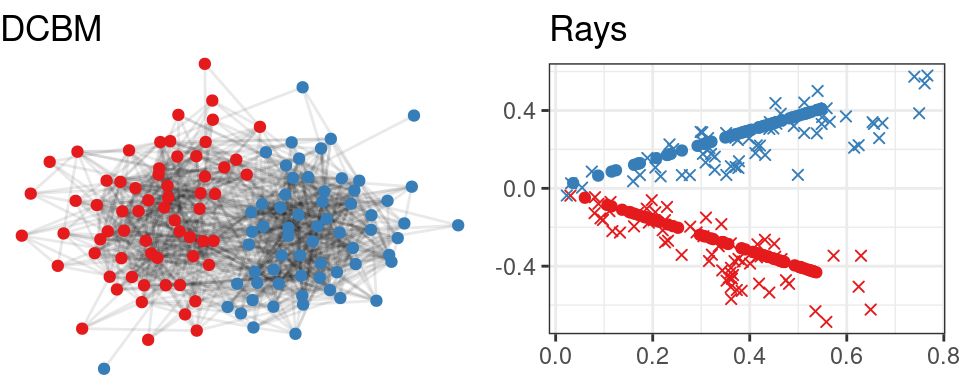
\includegraphics[width=0.5\linewidth]{slides_files/figure-beamer/unnamed-chunk-4-1} \end{center}

How might we cluster the nodes of a network?

\begin{enumerate}
\tightlist
\item
  Define a probability model with communities that might generate the
  graph (e.g., popularity adjusted block model).
\item
  Develop estimators for the parameters of the probability model,
  including the community labels.
\item
  Describe the properties of the estimators (e.g., consistency).
\end{enumerate}
\end{frame}

\begin{frame}{Bernoulli Graphs}
\protect\hypertarget{bernoulli-graphs}{}
Let \(G\) be an undirected and unweighted graph with \(n\) vertices.

\(G\) is described by adjacency matrix \(A\) such that
\(A_{ij} = \begin{cases} 1 & \text{an edge connects vertices } i \text{ and } j \\ 0 & \text{otherwise} \end{cases}\)

\(A_{ji} = A_{ij}\) and \(A_{ii} = 0\).

\vspace*{1\baselineskip}

\(A \sim \text{BernoulliGraph}(P)\) iff:

\begin{enumerate}
\tightlist
\item
  \(P\) is a matrix of edge probabilities between pairs of vertices.
\item
  \(A_{ij} \stackrel{\text{ind}}{\sim}\text{Bernoulli}(P_{ij})\) for
  each \(i < j\).
\end{enumerate}
\end{frame}

\begin{frame}{Block Models}
\protect\hypertarget{block-models}{}
Suppose each vertex \(v_1, ..., v_n\) has labels
\(z_1, ..., z_n \in \{1, ..., K\}\),\\
and each \(P_{ij}\) depends on labels \(z_i\) and \(z_j\).\\
Then \(A \sim \text{BernoulliGraph}(P)\) is a \emph{block model}.

\textbf{Example 1}: Stochastic Block Model with \(K=2\) communities.

\begin{columns}[T]
\begin{column}{0.48\textwidth}
\(P_{ij} = \begin{cases} p & z_i = z_j = 1 \\ q & z_i = z_j = 2 \\ r & z_i \neq z_j \end{cases}\)
\end{column}

\begin{column}{0.48\textwidth}
\begin{figure}

{\centering 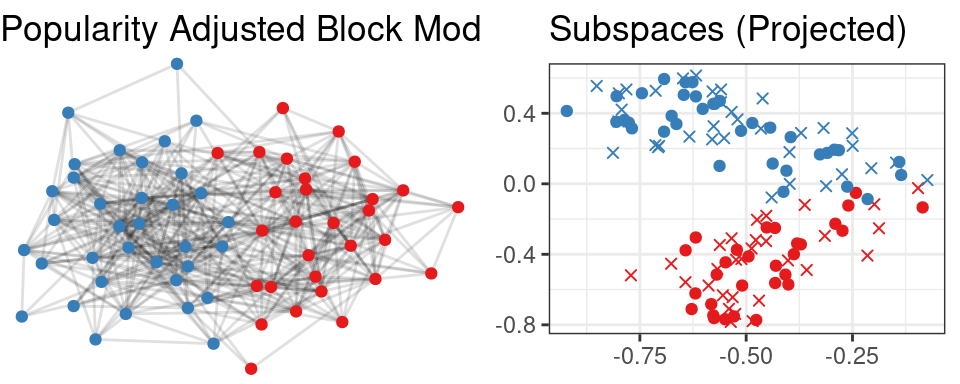
\includegraphics[width=1\linewidth]{slides_files/figure-beamer/unnamed-chunk-5-1} 

}

\caption{SBM with $p=1/2$, $q=1/4$, $r=1/8$}\label{unnamed-chunk-5}
\end{figure}
\end{column}
\end{columns}
\end{frame}

\begin{frame}{Popularity Adjusted Block Model}
\protect\hypertarget{popularity-adjusted-block-model}{}
\textbf{Def} Popularity Adjusted Block Model (Sengupta and Chen, 2017):

Let each vertex \(i \in [n]\) have \(K\) popularity parameters
\(\lambda_{i1}, ..., \lambda_{iK} \in [0, 1]\). Then
\(A \sim \text{PABM}(\{\lambda_{ik}\}_K)\) if each
\(P_{ij} = \lambda_{i z_j} \lambda_{j z_i}\).

\textbf{Def} (Noroozi, Rimal, and Pensky, 2020):

\(A\) is sampled from a PABM if \(P\) can be described as:

\begin{enumerate}
\tightlist
\item
  Let each \(P^{(kl)}\) denote the \(n_k \times n_l\) matrix of edge
  probabilities between communities \(k\) and \(l\).
\item
  Organize popularity parameters as vectors
  \(\lambda^{(kl)} \in \mathbb{R}^{n_k}\) such that
  \(\lambda^{(kl)}_i = \lambda_{k_i l}\) is the popularity parameter of
  the \(i\)\textsuperscript{th} vertex of community \(k\) towards
  community \(l\).
\item
  Each block can be decomposed as
  \(P^{(kl)} = \lambda^{(kl)} (\lambda^{(lk)})^\top\).
\end{enumerate}
\end{frame}

\begin{frame}{Generalized Random Dot Product Graph}
\protect\hypertarget{generalized-random-dot-product-graph}{}
\textbf{Def} Generalized Random Dot Product Graph\\
(Rubin-Delanchy, Cape, Tang, Priebe, 2020)

Let \(I_{p,q} = \text{blockdiag}(I_p, -I_q)\) and suppose that
\(x_1, \ldots, x_n \in \mathbb{R}^{p+q}\) are such that
\(x_i^\top I_{p,q} x_j \in [0,1]\).\\
Then \(A \sim \text{GRDPG}_{p, q}(X)\) iff
\(A \sim \text{BernoulliGraph}(X I_{p,q} X^\top)\), where
\(X = \begin{bmatrix} x_1 & \cdots & x_n \end{bmatrix}^\top\).

Adjacency Spectral Embedding (Sussman et al., 2012) estimates
\(x_1, ..., x_n \in \mathbb{R}^{p+q}\) from \(A\):

\begin{enumerate}
\tightlist
\item
  Let \(\hat{\Lambda}\) be the diagonal matrix that contains the
  absolute values of the \(p\) most positive and the \(q\) most negative
  eigenvalues.
\item
  Let \(\hat{V}\) be the matrix whose columns are the corresponding
  eigenvectors.
\item
  Compute \(\hat{X} = \hat{V} \hat{\Lambda}^{1/2}\).
\end{enumerate}

\textbf{Theorem}:
\(\max\limits_i \|\hat{X}_i - Q_n X_i \| = O_P \Big( \frac{(\log n)^c}{n^{1/2}} \Big)\)
as \(n \to \infty\)
\end{frame}

\begin{frame}{Connecting Block Models to the GRDPG Model}
\protect\hypertarget{connecting-block-models-to-the-grdpg-model}{}
All Bernoulli Graphs are GRDPGs.

\textbf{Example 1} (cont'd): SBM with \(K = 2\).

\begin{columns}[T]
\begin{column}{0.48\textwidth}
\[P_{ij} = \begin{cases} 
p & z_i = z_j = 1 \\
q & z_i = z_j = 2 \\
r & z_i \neq z_j
\end{cases}\]

\begin{center}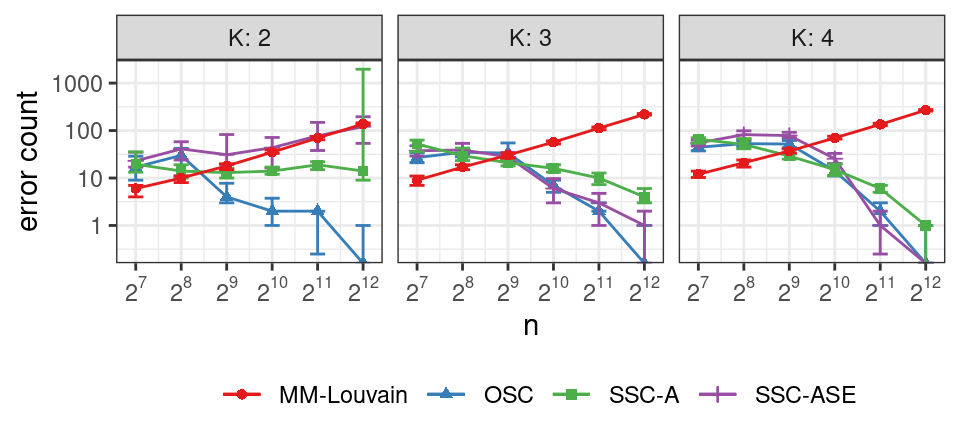
\includegraphics[width=1\linewidth]{slides_files/figure-beamer/unnamed-chunk-6-1} \end{center}
\end{column}

\begin{column}{0.48\textwidth}
\[P = 
\begin{bmatrix} 
P^{(11)} & P^{(12)} \\
P^{(21)} & P^{(22)}
\end{bmatrix} =
X I_{2,0} X^\top\]

\[X = \begin{bmatrix} 
\sqrt{p} & 0 \\
\vdots & \vdots \\
\sqrt{p} & 0 \\
\sqrt{r^2 / p} & \sqrt{q - r^2 / p} \\
\vdots & \vdots \\
\sqrt{r^2 / p} & \sqrt{q - r^2 / p}
\end{bmatrix}\]
\end{column}
\end{columns}
\end{frame}

\begin{frame}{Connecting Block Models to the GRDPG Model}
\protect\hypertarget{connecting-block-models-to-the-grdpg-model-1}{}
\textbf{Example 1} (cont'd): To perform community detection,

\begin{enumerate}
\tightlist
\item
  Note that \(A\) is a RDPG because \(P = X X^\top\).
\item
  Compute the ASE \(A \approx \hat{X} \hat{X}^\top\) with
  \(\hat{X} = \hat{V} \hat{\Lambda}^{1/2}\).
\item
  Apply a clustering algorithm (e.g., \(K\)-means) to \(\hat{X}\),\\
  noting that \(\hat{X}\) approaches point masses as \(n \to \infty\).
\end{enumerate}

\begin{center}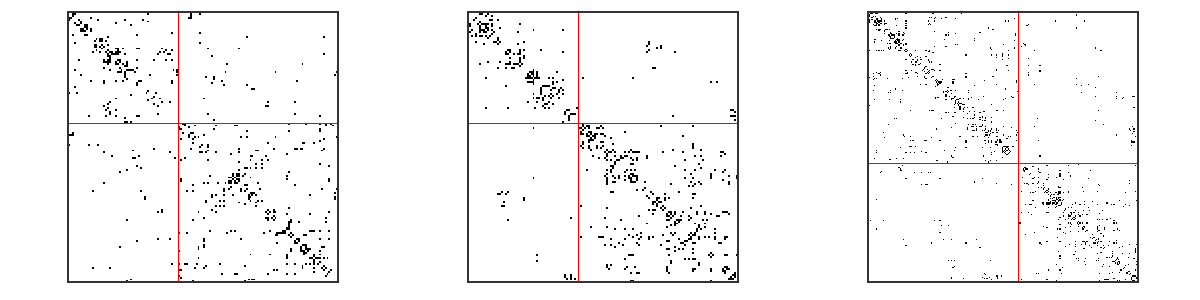
\includegraphics[width=0.5\linewidth]{slides_files/figure-beamer/unnamed-chunk-7-1} \end{center}
\end{frame}

\begin{frame}{Connecting Block Models to the GRDPG Model}
\protect\hypertarget{connecting-block-models-to-the-grdpg-model-2}{}
\begin{columns}[T]
\begin{column}{0.48\textwidth}
\begin{center}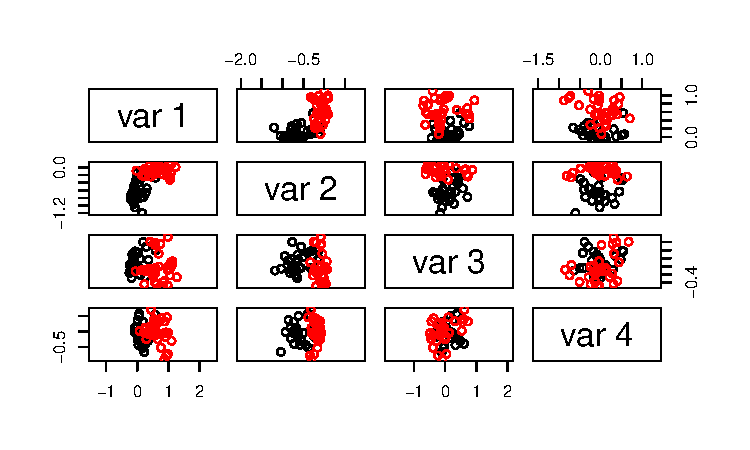
\includegraphics[width=1\linewidth]{slides_files/figure-beamer/unnamed-chunk-8-1} \end{center}
\end{column}

\begin{column}{0.48\textwidth}
\vspace*{0\baselineskip}

\begin{center}\includegraphics[width=1\linewidth]{slides_files/figure-beamer/unnamed-chunk-9-1} \end{center}
\end{column}
\end{columns}
\end{frame}

\begin{frame}{Connecting the PABM to the GRDPG}
\protect\hypertarget{connecting-the-pabm-to-the-grdpg}{}
\textbf{Theorem} (KTT): \(A \sim \text{PABM}(\{\lambda_{ik}\}_K)\) is
equivalent to \(A \sim \text{GRDPG}_{p, q}(X U)\) with

\begin{itemize}
\tightlist
\item
  \(p = K (K + 1) / 2\), \(q = K (K - 1) / 2\);
\item
  \(U\) is an orthogonal matrix;
\item
  \(X \in \mathbb{R}^{n \times K^2}\) is a block diagonal matrix
  composed of popularity vectors with each block corresponding to a
  community.
\end{itemize}

\[X = \begin{bmatrix}
\Lambda^{(1)} & \cdots & 0 \\
0 & \ddots & 0 \\
0 & \cdots & \Lambda^{(K)}
\end{bmatrix} 
\in \mathbb{R}^{n \times K^2}\]

\[\Lambda^{(k)} = \begin{bmatrix} 
\lambda^{(k1)} & \cdots & \lambda^{(kK)} 
\end{bmatrix} 
\in \mathbb{R}^{n_k \times K}\]

\[A \sim \text{PABM}(\{\lambda_{ik}\}_K) \text{ iff } A \sim \text{GRDPG}_{p, q}(X U)\]
\end{frame}

\begin{frame}{Orthogonal Spectral Clustering}
\protect\hypertarget{orthogonal-spectral-clustering}{}
\textbf{Theorem} (KTT): If \(P = V \Lambda V^\top\) and
\(B = n V V^\top\),\\
then \(B_{ij} = 0\) if \(z_i \neq z_j\).

\textbf{Algorithm}: Orthogonal Spectral Clustering:

\begin{enumerate}
\tightlist
\item
  Let \(V\) be the eigenvectors of \(A\) corresponding to the
  \(K (K+1)/2\) most positive and \(K (K-1) / 2\) most negative
  eigenvalues.
\item
  Compute \(B = |n V V^\top|\) applying \(|\cdot|\) entry-wise.
\item
  Construct graph \(G\) using \(B\) as its similarity matrix.
\item
  Partition \(G\) into \(K\) disconnected subgraphs.
\end{enumerate}

\textbf{Theorem} (KTT): Let \(\hat{B}\) with entries \(\hat{B}_{ij}\) be
the affinity matrix from OSC. Then \(\forall\) pairs \((i, j)\)
belonging to different communities and sparsity factor satisfying
\(n \rho_n = \omega\big((\log n)^{4c}\big)\),\\
\(\max_{i, j} \hat{B}_{ij} = O_P \Big( \frac{(\log n)^c}{\sqrt{n \rho_n}} \Big)\)
as \(n \to \infty\).
\end{frame}

\begin{frame}{Simulation Results}
\protect\hypertarget{simulation-results}{}
We compare four algorithms for community detection on randomly generated
PABMs:

\begin{itemize}
\tightlist
\item
  Modularity Maximization (Sengupta and Chen) using the Louvain
  algorithm;
\item
  Orthogonal Spectral Clustering (KTT);
\item
  Sparse Subspace Clustering on the columns of \(A\)\\
  (Noorozi, Rimal, Pensky);
\item
  Sparse Subspace Clustering on the ASE (KTT).
\end{itemize}

\begin{center}\includegraphics[width=1\linewidth]{slides_files/figure-beamer/unnamed-chunk-10-1} \end{center}
\end{frame}

\begin{frame}{Additional Slides}
\protect\hypertarget{additional-slides}{}
\end{frame}

\begin{frame}{Simulation Setup}
\protect\hypertarget{simulation-setup}{}
\begin{enumerate}
\tightlist
\item
  \(z_1, ..., z_n \stackrel{\text{iid}}{\sim}\text{Categorical}(1/K, ..., 1/K)\)
\item
  \(\lambda_{ik} \stackrel{\text{iid}}{\sim}\text{Beta}(a_{ik}, b_{ik})\)

  \begin{itemize}
  \tightlist
  \item
    \(a_{ik} = \begin{cases} 2 & z_i = k \\ 1 & z_i \neq k \end{cases}\)
  \item
    \(b_{ik} = \begin{cases} 1 & z_i = k \\ 2 & z_i \neq k \end{cases}\)
  \end{itemize}
\item
  \(P_{ij} = \lambda_{i z_j} \lambda_{j z_i}\)
\item
  \(A \sim \text{BernoulliGraph}(P)\)
\end{enumerate}
\end{frame}

\begin{frame}{Future Work}
\protect\hypertarget{future-work}{}
\end{frame}

\end{document}
